% Created 2023-02-07 Tue 01:43
% Intended LaTeX compiler: pdflatex
\documentclass[11pt]{article}
\usepackage[utf8]{inputenc}
\usepackage[T1]{fontenc}
\usepackage{graphicx}
\usepackage{longtable}
\usepackage{wrapfig}
\usepackage{rotating}
\usepackage[normalem]{ulem}
\usepackage{amsmath}
\usepackage{amssymb}
\usepackage{capt-of}
\usepackage{hyperref}
\usepackage[polish, american]{babel}
\usepackage[margin=3cm]{geometry}
\newgeometry{vmargin={5mm}, hmargin={20mm,20mm}}
\author{placeholder}
\date{\today}
\title{Przykladowyegzamin}
\hypersetup{
 pdfauthor={placeholder},
 pdftitle={Przykladowyegzamin},
 pdfkeywords={},
 pdfsubject={},
 pdfcreator={Emacs 30.0.50 (Org mode 9.6)}, 
 pdflang={English}}
\begin{document}

\maketitle
\tableofcontents

\section{[8/10] Algebra}
\label{sec:orgfc8b25d}
\subsection{{\bfseries\sffamily DONE} Zad 1}
\label{sec:orga056ef7}
\begin{align*}
\Im \left(\frac{1+3i}{3-2i} + i^{3} + 5\right)
 &=\Im \left(\frac{1+3i}{3-2i} + \frac{i^{3}(3-2i)}{3-2i} + \frac{5(3-2i)}{3-2i}\right)\\
 &= \Im \left(\frac{1+3i + 3i^3 - 2 i^4 + 15 - 10i}{3-2i}\right)\\
 &= \Im \left(\frac{16 - 7i + 3i^{3} -2i^{4}}{3-2i}\right)\\
 &= \Im \left(\frac{14 - 10i}{3-2i}\right)\\
 &= \Im \left(\frac{14 - 10i}{3-2i} \cdot \frac{3+2i}{3+2i}\right)\\
 &= \Im \left(\frac{42 + 28i - 30i + 20}{9 + 4}\right)\\
 &= \Im \left(\frac{62 - 2i }{13}\right)\\
 &= \frac{-2}{13}
\end{align*}
\subsection{{\bfseries\sffamily DONE} Zad 2}
\label{sec:org4c8c1f8}
\begin{align*}
  \frac{ { (3 - 3i)}^{14} }
  { { (-1+i\sqrt{3}) }^{11} }
  &= \frac{z^{14}}{w^{11}}
\end{align*}
\subsubsection{\(z\)}
\label{sec:org713ef66}
$$\sin(\varphi_z) = \frac{-3}{3\sqrt{2}}
 = \frac{-1}{\sqrt{2}}
 = \frac{-\sqrt{2}}{2} \to \varphi_z = \frac{7}{4}\pi$$

\begin{align*}
  z^{14} &= {(3 - 3i)}^{14}\\
  &= {(3-3i)}^{14}\\
  &= {(3\sqrt{2})}^{14}(\cos 14 \varphi + i \sin 14 \varphi)\\
  &= {(3\sqrt{2})}^{14} \left(\cos \left(14 \cdot \frac{7}{4} \pi \right) + i \sin \left(14 \cdot \frac{7}{4} \pi \right) \right)\\
  &= {(3\sqrt{2})}^{14} \left( \cos \left ( \frac{49}{2} \pi \right) + i \sin \left(\frac{49}{2} \pi \right) \right)\\
  &= {(3\sqrt{2})}^{14} \left( \cos \left ( \frac{1}{2} \pi \right) + i \sin \left(\frac{1}{2} \pi \right) \right)\\
  &= {(3\sqrt{2})}^{14} ( 0 + i 1 )\\
  &= {(3\sqrt{2})}^{14}i
\end{align*}
\subsubsection{\(w\)}
\label{sec:orgb1910ac}
$$\sin(\varphi_w) = \frac{\sqrt{3}}{\sqrt{4}} = \frac{\sqrt{3}}{2}
\to \varphi_w = \frac{2}{3} \pi$$

\begin{align*}
w^{11} &= 2^{11} \left( \cos \left(11 \cdot \frac{2}{3} \pi \right)
+ i \sin \left( 11 \cdot \frac{2}{3} \pi \right) \right)\\
&= 2^{11} \left( -\cos \frac{\pi}{3}
- i \sin \frac{\pi}{3} \right)\\
&= 2^{11} \left(- \frac{1}{2} - i \frac{\sqrt{3}}{2} \right)\\
&= 2^{10} \left(-1 - i \sqrt{3} \right)
\end{align*}
\subsubsection{Podstawiamy}
\label{sec:orge918c8f}
\begin{align*}
\frac{ { (3 - 3i)}^{14} }
{ { (-1+i\sqrt{3}) }^{11} }
&= \frac{z^{14}}{w^{11}}\\
&=\frac{(3\sqrt{2})^{14} i }
{2^{10}(-1 -i\sqrt{3})}\\
&=\frac{ ((3\sqrt{2})^{14} i)(-1 + i\sqrt{3}) }
{2^{10}(-1 -i\sqrt{3})(-1 + i\sqrt{3})}\\
&=\frac{ ((3\sqrt{2})^{14} i)(-1 + i\sqrt{3}) }
{2^{10}(-2)}\\
&=\frac{ ((3\sqrt{2})^{14} i)(-1 + i\sqrt{3}) }
{-2^{11}}
\end{align*}
\subsection{{\bfseries\sffamily DONE} Zad 3}
\label{sec:org45ebf0e}
Wyznacznik macierzy głownej \(= 20\).
\\\empty
\(A = \begin{bmatrix}
3  & -2 & 1 & 0 \\
2  & -1 & 3 & 1 \\
2 & -1 & 3 & 4 \\
0 & 1 & 3 & -1 \\
\end{bmatrix}\),
\(X = \begin{bmatrix}
4\\
1\\
-2\\
3
\end{bmatrix}\)
\subsubsection{{\bfseries\sffamily DONE} \(A_4\)}
\label{sec:org49080de}
\begin{align*}A_4 &= \begin{vmatrix}
                       3  & -2 & 1 & 4 \\
                       2  & -1 & 3 & 1 \\
                       2 & -1 & 3 & -2 \\
                       0 & 1 & 3 & 3 \\
                     \end{vmatrix}
  \xrightarrow[k_3 = k_3 - k4]{k_4 = k_4 - 3k_2}
  \begin{vmatrix}
    3 & -2 & -3  & 10 \\
    2 & -1 &  2  & 4 \\
    2 & -1 & 5   & 1 \\
    0 & 1  & 0   & 0 \\
  \end{vmatrix}\\
                  &= 1 \cdot (-1)^{6} \cdot \begin{vmatrix}
                                              3 & -3 & 10 \\
                                              2 & 2  & 4  \\
                                              2 & 5  & 1\\
                                              \end{vmatrix}\\
                  &=1 \cdot (6 + 100 - 24) - (40 + 60 -6)\\
                  &=82 - 94\\
                  &= - 12
\end{align*}
\subsubsection{{\bfseries\sffamily DONE} Podstawianie}
\label{sec:org9883acb}
$$x_4 = \frac{-12}{20} = \frac{-3}{5}$$
\subsection{{\bfseries\sffamily DONE} Zad 4}
\label{sec:org8efb3fd}
\begin{align*}
  \left[
  \begin{array}{cccc|c}
    3  & -2 & 1 & 0 & 4\\
    2  & -1 & 3 & 1 & 1 \\
    2 & -1 & 3 & 4  & -2\\
    x_1 & x_2 & x_3 & x_4  & y\\
  \end{array}
  \right]
  \xrightarrow[w_{1} = w_{1} - w_{2}]{}
       & \left[
         \begin{array}{cccc|c}
           1  & -1 & -2 & -1 & 3\\
           2  & -1 & 3 & 1 & 1 \\
           2 & -1 & 3 & 4  & -2\\
           x_1 & x_2 & x_3 & x_4  & y\\
         \end{array}
  \right]
  \\
  \xrightarrow[w_{2} = w_{2} - 2 w_{1} ]{w_3 = w_3 - 2 w_1}
       & \left[
         \begin{array}{cccc|c}
           1  & -1 & -2 & -1 & 3\\
           0  & 1 & 7 & 3 & -5 \\
           0 & 1 & 7  & 6 & -8 \\
           x_1 & x_2 & x_3 & x_4  & y\\
         \end{array}
  \right]
  \\
  \xrightarrow[w_{3} = w_{3} - w_{2}]{w_{1} = w_{1} + w_{2}}
       &\left[
         \begin{array}{cccc|c}
           1 & 0 & 5 & 2 & -2\\
           0 & 1 & 7 & 3 & -5\\
           0 & 0 & 0 & 3 & -3\\
           x_1 & x_2 & x_3 & x_4  & y\\
         \end{array}
  \right]
  \\
  \xrightarrow[k_{4} = k_{3}]{k_{3} = k_{4}}
       &\left[
         \begin{array}{cccc|c}
           1 & 0 & 2 & 5 & -2\\
           0 & 1 & 3 & 7 & -5\\
           0 & 0 & 3 & 0 & -3\\
           x_1 & x_2 & x_4 & x_3  & y\\
         \end{array}
  \right]
  \\
  \xrightarrow[w_{3} = w_{3} \cdot \frac{1}{3}]{}
       &\left[
         \begin{array}{cccc|c}
           1 & 0 & 2 & 5 & -2\\
           0 & 1 & 3 & 7 & -5\\
           0 & 0 & 1 & 0 & -1\\
           x_1 & x_2 & x_4 & x_3  & y\\
         \end{array}
  \right]
  \\
  \xrightarrow[w_{2} = w_{2} - 3 \cdot w_{3}]{w_1 = w_1 - 2 \cdot w_3}
       &\left[
         \begin{array}{cccc|c}
           1 & 0  & 0 & 5 & 0\\
           0 & 1  & 0 & 7 & -2\\
           0 & 0 & 1 & 0 & -1\\
           x_1 & x_2 & x_4 & x_3  & y\\
         \end{array}
  \right]
\end{align*}
\(x_1 = -5 x_3\)
\\\empty
\(x_2 = -7x_3 -2\)
\\\empty
\(x_3 \in \mathbb{R}\)
\\\empty
\(x_4 = -1\)
\subsection{{\bfseries\sffamily DONE} Zad 5}
\label{sec:orgda233af}
$$XA = B \xrightarrow[\text{prawostronnie } A^{-1}]{} X A A^{-1} = BA^{-1} \to X = B A^{-1}$$
\(A = \begin{bmatrix}
       1 & 2 & -3 \\
       3 & 0 & -2 \\
       -1 & -4 & 5\\
     \end{bmatrix}\),
     \(B= \begin{bmatrix}
     4 & 2 & -5\\
     3 & 0 & -2\\
     \end{bmatrix}\)

\(\det A = (36 + 4) - (8 + 30) = 40 - 38 = 2\)
\begin{align*}
  A^{-1} &= \frac{1}{2} \begin{bmatrix}
                          &\begin{vmatrix}
                             0 & -2\\
                             -4 & 5\\
                           \end{vmatrix}
                          &- \begin{vmatrix}
                               3 & -2 \\
                               -1 & 5 \\
                             \end{vmatrix}
                          &\begin{vmatrix}
                             3 & 0 \\
                             -1 & -4\\
                           \end{vmatrix}
                          \\
                          &- \begin{vmatrix}
                               2 & -3 \\
                               -4 & 5 \\
                             \end{vmatrix}
                          &\begin{vmatrix}
                             1 & -3\\
                             -1 & 5 \\
                           \end{vmatrix}
                          &- \begin{vmatrix}
                               1 & 2 \\
                               -1 & -4\\
                             \end{vmatrix}
                          \\
                          &\begin{vmatrix}
                             2 & -3\\
                             0 & -2 \\
                           \end{vmatrix}
                          &- \begin{vmatrix}
                               1 & -3 \\
                               3 & -2\\
                             \end{vmatrix}
                          &\begin{vmatrix}
                             1 & 2\\
                             3 & 0\\
                           \end{vmatrix}
                        \end{bmatrix}^{T}
  \\
         &=\frac{1}{2}
           \begin{bmatrix}
             -8 & -13 & -12\\
             2 & 2 & 2\\
             -4 & -7 & -6\\
           \end{bmatrix}^{T}
\\
         &=\frac{1}{2}
           \begin{bmatrix}
             -8 &  2 & -4\\
             -13 & 2 & -7\\
             -12 & 2 & -6\\
           \end{bmatrix}
  \\
         &= \begin{bmatrix}
              -4 & 1 & -2\\
              -\frac{13}{2} & 1 & - \frac{7}{2}\\
              -6 & 1 & -3\\
            \end{bmatrix}
\end{align*}
\begin{align*}
  X = BA^{-1} &= \begin{bmatrix}
                   4 & 2 & -5\\
                   3 & 0 & -2\\
                 \end{bmatrix}
  \begin{bmatrix}
    -4 & 1 & -2\\
    -\frac{13}{2} & 1 & - \frac{7}{2}\\
    -6 & 1 & -3\\
  \end{bmatrix}
  \\
              &= \begin{bmatrix}
                   -16 - 13 + 30 & 4 + 2 - 5 & - 8 - 7 + 15\\
                   -12 + 0 + 12  & 3 + 0 - 2 & - 6 +0 +6 \\
                 \end{bmatrix}
  \\
              &= \begin{bmatrix}
                   1 & 1 & 0\\
                   0 & 1 & 0\\
                 \end{bmatrix}
\end{align*}
\subsection{{\bfseries\sffamily DONE} Zad 6}
\label{sec:org91b77a9}
Macierz obrotu o kąt \(\displaystyle\frac{\pi}{3}\) w kierunku dodatnim
\(A = \begin{bmatrix}
\cos \frac{\pi}{3} & -\sin \frac{\pi}{3}\\
\sin \frac{\pi}{3} & \cos \frac{\pi}{3}\\
\end{bmatrix}\).
\subsubsection{{\bfseries\sffamily DONE} Związek między współrzędnymi \(x_1, x_2\) w bazie \(\vec{e}_1, \vec{e}_2\) a współrzędnymi \(\hat{x}_1, \hat{x}_2\) w bazie \(\vec{u}, \vec{v}\).}
\label{sec:orgdb8fbdb}
\begin{align*}
  \vec{u} &= A \cdot \vec e_{1}
  \\
          &=
            \begin{bmatrix}
              \cos \frac{\pi}{3} & -\sin \frac{\pi}{3}\\
              \sin \frac{\pi}{3} & \cos \frac{\pi}{3}\\
            \end{bmatrix}
  \begin{bmatrix}
    1 \\
    0 \\
  \end{bmatrix}
  \\
          &= \begin{bmatrix}
               \frac{1}{2}\\
               \frac{\sqrt{3}}{2}\\
             \end{bmatrix}
\end{align*}

\begin{align*}
  \vec{v} &= A \cdot \vec e_{2}
  \\
          &=
            \begin{bmatrix}
              \cos \frac{\pi}{3} & -\sin \frac{\pi}{3}\\
              \sin \frac{\pi}{3} & \cos \frac{\pi}{3}\\
            \end{bmatrix}
  \begin{bmatrix}
    0 \\
    1 \\
  \end{bmatrix}
  \\
          &= \begin{bmatrix}
               -\frac{\sqrt{3}}{2}\\
               \frac{1}{2}\\
             \end{bmatrix}
\end{align*}
\subsubsection{{\bfseries\sffamily DONE} Znalesć współrzędne wektora \(\vec{x}\) w bazie \(\vec u, \vec v\), jeżeli jego współrzędne w bazie \(\vec e_1, \vec e_2\) wynoszą: \(1, -2\).}
\label{sec:orgda9450b}
\(\vec x = \begin{bmatrix}
            1 \\
            -2
          \end{bmatrix}_{\vec e_1, \vec e_2}\)
\begin{align*}
  \begin{bmatrix}
    \hat x_{1} \\
    \hat x_{2} \\
  \end{bmatrix}
  &= A^{T} \cdot
    \begin{bmatrix}
      x_{1}\\
      x_{2}\\
    \end{bmatrix}
  \\
  &= \begin{bmatrix}
       \cos \frac{\pi}{3} & \sin \frac{\pi}{3}\\
       \sin \frac{\pi}{3} & \cos \frac{\pi}{3}\\
     \end{bmatrix}^{T}
    \begin{bmatrix}
      x_{1}\\
      x_{2}\\
    \end{bmatrix}
  \\
  &= \begin{bmatrix}
       \frac{1}{2} &  \frac{\sqrt{3}}{2}\\
       \frac{-\sqrt{3}}{2} & \frac{1}{2}\\
     \end{bmatrix}
    \begin{bmatrix}
      1\\
      -2\\
    \end{bmatrix}
  \\
  &= \begin{bmatrix}
       \frac{1}{2} - \sqrt{3}\\
       -\frac{\sqrt{3}}{2} - 1\\
     \end{bmatrix}
  \\
  &= \begin{bmatrix}
       \frac{1 - 2\sqrt{3}}{2}\\
       \frac{- 2 - \sqrt{3}}{2}\\
    \end{bmatrix}
\end{align*}
\begin{enumerate}
\item Sporządzić rysunek
\label{sec:orgdfe831e}
\begin{center}
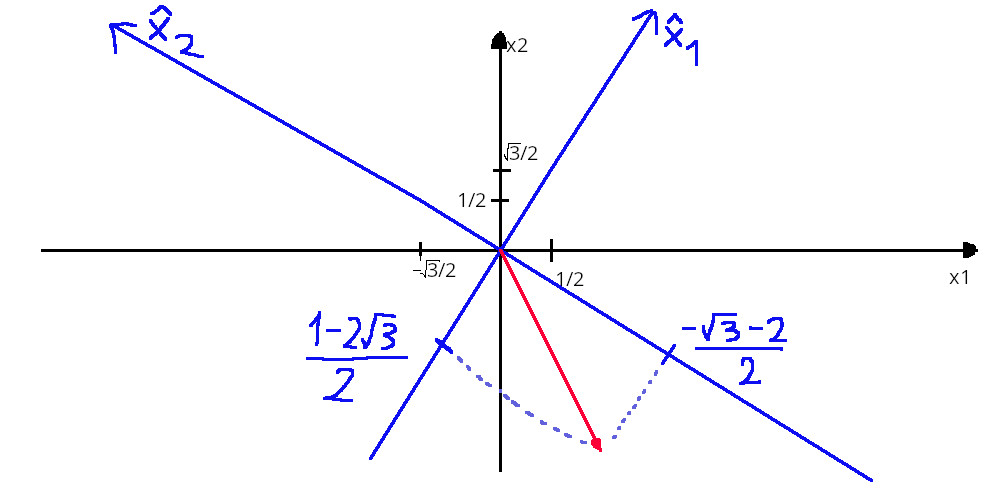
\includegraphics[width=.9\linewidth]{img/zad6.jpg}
\end{center}
\end{enumerate}
\subsection{{\bfseries\sffamily TODO} Zad 7}
\label{sec:orga75d0c9}
\subsubsection{{\bfseries\sffamily PROJ} Zad 7a}
\label{sec:org21ee526}
\[-72 + 13 x^{2} - 10xy + 13y^{2} = 0\]
Forma kwadratowa:
\[A = \begin{bmatrix}
        13 & -5\\
        -5 & 13\\
      \end{bmatrix}\]
\[\det A = 13^2 - {(-5)}^{2}
  = 169 - 25
  = 144\]
Typ elptyczny
\begin{enumerate}
\item {\bfseries\sffamily DONE} Znaleść wartości własne \(\lambda\)
\label{sec:orge4cfbc0}
\[A (I\lambda) = \begin{bmatrix}
        13 - \lambda & -5\\
        -5 & 13 - \lambda \\
      \end{bmatrix}\]
\begin{align*}
  {(13 - \lambda)}^{2} - 25 &= 0\\
  169 - 26 \lambda + {\lambda}^{2} - 25 &= 0 \\
  {\lambda}^{2} - 26 \lambda + 144 &= 0\\
\end{align*}
\[\Delta = 26^{2} - 4 \cdot 144 = 676 - 576 = 100\]
\[\sqrt{\Delta} = 10\]
\[\lambda_1 = \frac{-b + \sqrt{\Delta}}{2a}
= \frac{26 + 10}{2} = 18\]
\[\lambda_2 = \frac{-b - \sqrt{\Delta}}{2a}
= \frac{26 - 10}{2} = 8\]
\item {\bfseries\sffamily DONE} Wersory
\label{sec:org247fa08}
\begin{enumerate}
\item Dla \(\lambda_1\)
\label{sec:org25f8af3}
\[\begin{bmatrix}
  13 - 18 & -5\\
  -5 & 13 - 18\\
\end{bmatrix}
=
\begin{bmatrix}
  -5 & -5\\
  -5 & -5\\
\end{bmatrix}\]
\[\begin{bmatrix}
    -5 & -5\\
    -5 & -5\\
  \end{bmatrix}
  \begin{bmatrix}
    v_{11}\\
    v_{12}\\
  \end{bmatrix} = \begin{bmatrix}
                    0\\
                    0\\
                  \end{bmatrix}\]
\begin{enumerate}
\item Wyznaczyć \(W_{1}\)
\label{sec:orgc5e4c05}
\begin{align*}
-5 v_{11} -5 v_{12} &= 0 && / -5\\
   v_{11} + v_{12} &= 0\\
   v_{11} &= - v_{12}
\end{align*}
\[\vec V_{1} = \begin{bmatrix}
                 v_{11}\\
                 v_{12}
               \end{bmatrix}
               = \begin{bmatrix}
                   -v_{12}\\
                   v_{12}\\
                 \end{bmatrix}\]
Trzeba będzie zamienić \(W_{1}\) i \(W_{2}\), bo wyszedł \(-\) u góry.
\[|\vec{V}_{1}| = \sqrt{ {(-v_{12})}^{2} + v_{12}^{2}}
  = \sqrt{ v_{12}^{2} + v_{12}^{2}}
    = \sqrt{ 2 v_{12}^{2} }
    = \sqrt{2} v_{12}\]
\[\vec W_1 = \begin{bmatrix}
               \displaystyle\frac{-v_{12}}{\sqrt{2} v_{12}}\\
               \displaystyle\frac{v_{12}}{\sqrt{2} v_{12}}\\
             \end{bmatrix}
             = \begin{bmatrix}
                 \frac{-1}{\sqrt{2}}\\
                 \frac{1}{\sqrt{2}}\\
               \end{bmatrix}
               = \begin{bmatrix}
                   \frac{-\sqrt{2}}{2}\\
                   \frac{\sqrt{2}}{2}\\
                 \end{bmatrix}\]
\end{enumerate}
\item Dla \(\lambda_2\)
\label{sec:orgc4467e1}
\[\begin{bmatrix}
  13 - 8 & -5\\
  -5 & 13 - 8\\
\end{bmatrix}
=
\begin{bmatrix}
  5 & -5\\
  -5 & 5\\
\end{bmatrix}\]
\[\begin{bmatrix}
    5 & -5\\
    -5 & 5\\
  \end{bmatrix}
  \begin{bmatrix}
    v_{21}\\
    v_{22}\\
  \end{bmatrix} = \begin{bmatrix}
                    0\\
                    0\\
                  \end{bmatrix}\]
\begin{enumerate}
\item Wyznaczyc \(W_{2}\)
\label{sec:org4b60d66}
\begin{align*}
  5 v_{21} - 5 v_{22} &= 0 && / 5\\
  v_{21} - v_{22} &= 0 \\
  v_{21} = v_{22}
\end{align*}
\[\vec V_{2} = \begin{bmatrix}
                 v_{22}\\
                 v_{22}
               \end{bmatrix}\]
\[| \vec V_{2} | = \sqrt{ v_{22}^{2} + v_{22}^{2}}
  = \sqrt{2 v_{22}^{2}}
  = \sqrt{2} v_{22}\]
\[\vec W_2 = \begin{bmatrix}
               \displaystyle\frac{v_{22}}{\sqrt{2} v_{22}}\\
               \displaystyle\frac{v_{22}}{\sqrt{2} v_{22}}\\
             \end{bmatrix}
             = \begin{bmatrix}
                 \frac{1}{\sqrt{2}}\\
                 \frac{1}{\sqrt{2}}\\
               \end{bmatrix}
               = \begin{bmatrix}
                   \frac{\sqrt{2}}{2}\\
                   \frac{\sqrt{2}}{2}\\
                 \end{bmatrix}\]
\end{enumerate}
\end{enumerate}
\item {\bfseries\sffamily DONE} Macież obrotu
\label{sec:orgfe01950}
Zamieniamy kolejność wersorów bo minus ma być w lewym górnym.
\[\begin{bmatrix}
x_{1}\\
x_{2}\\
\end{bmatrix} =\begin{bmatrix}
\frac{\sqrt{2}}{2} & -\frac{\sqrt{2}}{2}\\
\frac{\sqrt{2}}{2} & \frac{\sqrt{2}}{2}\\
\end{bmatrix}  \begin{bmatrix}
\hat{x}_{1}\\
\hat{x}_{2}\\
\end{bmatrix}\]
\[x_1 = \frac{\sqrt{2}}{2} \hat{x}_{1} - \frac{\sqrt{2}}{2} \hat{x}_2\]
\[x_2 = \frac{\sqrt{2}}{2} \hat{x}_{1} + \frac{\sqrt{2}}{2} \hat{x}_2\]
\textbf{Zwijamy}
\begin{align*}
  8 \hat{x}_1^2 + 18 \hat{x}_2^2 -72 &= 0 && / 72\\
  \frac{\hat{x}_{1}^{2}}{3^{2}} + \frac{\hat{x}_{2}^{2}}{2^{2}} &= 1
\end{align*}
\item {\bfseries\sffamily TODO} wykres
\label{sec:orgb07b395}
\end{enumerate}
\subsection{{\bfseries\sffamily DONE} Zad 8}
\label{sec:orga7fd048}
\begin{align*}
A&=(0,1,5),& B&=(-2,3,1),& C&=(-2, 7,3)
\end{align*}
\(|AB| = \sqrt{(-2)^{2} + (3-1)^{2} + (5 -1)^{2}} = \sqrt{4 + 4 +16} = \sqrt{24} = 2\sqrt{6}\)
\\\empty
\(|AC| = \sqrt{ 4 + 36 + 4} = \sqrt{44} = 2 \sqrt{11}\)
\\\empty
\(|BC| = \sqrt{0 + 16 + 4} = \sqrt{20} = 2\sqrt{5}\)
\subsubsection{{\bfseries\sffamily DONE} Rówanie prostej w postaci kanonicznej}
\label{sec:orgeed9170}
$$\frac{x - 0}{-2 - 0} = \frac{y - 1}{7 - 1} = \frac{z - 5}{3 -5}
\to \frac{x - 0}{-2} = \frac{y - 1}{6} = \frac{z - 5}{-2}
= t$$
\subsubsection{{\bfseries\sffamily DONE} Równanie prostej w postaci paraetrycznej}
\label{sec:org60489dc}
\[\begin{cases}
x-0 = -2t \to & x = -2t\\
y - 1 = 6t \to & y = 6t +1\\
z -5 = -2t \to & z = -2t + 5\\
\end{cases}\]
\subsubsection{{\bfseries\sffamily DONE} Oblcizanie odległości punktu od prostej}
\label{sec:org368b0fe}
\begin{align*}
  \overrightarrow{BD} \times \vec{k}
  &= \begin{vmatrix}
       \vec{i} & \vec{j} & \vec{k}\\
       2 & -2 & 4\\
       -2 & 6 & -2\\
     \end{vmatrix}
  \\
  &= (4\vec{i} + 12\vec{k} - 8 \vec{j}) - (4 \vec{k} + 24 \vec{i} - 4 \vec{j})
  \\
  &= 4\vec{i} + 12\vec{k} - 8 \vec{j} - 4 \vec{k} - 24 \vec{i} + 4 \vec{j}
  \\
  &= -20\vec{i} - 4\vec{j} + 8 \vec{k}
\end{align*}
\(B=(-2,3,1)\)
\\\empty
\(D=(0, 1, 5)\)
\\\empty
wektor kierunkowy: \(\vec{k} = [-2, 6, -2]\)
\\\empty
\(\overrightarrow{BD} = [0 + 2 , 1 - 3 ,5 -1] = [2, -2, 4]\)
\\\empty
$$|BD| = \frac{|\overrightarrow{BD}|}{|\vec{k}|}
= \frac{\sqrt{(-20)^{2} + 4^{2} + 8^{2}}}
{\sqrt{(-2)^{2} + 6^{2} + (-2)^{2}} }
= \frac{\sqrt{400 + 16 + 64}}{\sqrt{4 + 36 + 4}}
= \frac{\sqrt{480}}{\sqrt{44}}
= \sqrt{\frac{120}{11}}
= \frac{\sqrt{120}}{\sqrt{11}}$$
\subsubsection{{\bfseries\sffamily DONE} Obliczanie pola trójkąta}
\label{sec:orgbe2776b}
$$P = \frac{ 2\sqrt{11} \cdot\frac{ \sqrt{120} }{\sqrt{11}} }
{2}
= \frac{2\sqrt{120}}{2}
= \sqrt{120}
= 2\sqrt{30}$$
\subsection{{\bfseries\sffamily DONE} Zad 9}
\label{sec:org9609595}
Płaszczyzna: \(\pi : x - y + z - 2 = 0\)
\\\empty
Postać krawędziowa prostej:
\(l_1 : \begin{cases}
3x + 2y - z - 4 = 0\\
-x - 2y + z + 2 = 0
\end{cases}\)
\subsubsection{{\bfseries\sffamily DONE} Wyznaczyć wektor kierunkowy porstej}
\label{sec:org84c1ec6}
\begin{align*}
  \vec k &= \begin{vmatrix}
              \vec i & \vec j & \vec k\\
              3 & 2 & -1 \\
              -1 & -2 & 1\\
            \end{vmatrix}
  \\
         &= 2 \vec i - 6 \vec k + 1 \vec j - (-2 \vec k + 2 \vec i + 3 \vec j)
  \\
         &= [0, -2, -4]
\end{align*}
\subsubsection{{\bfseries\sffamily DONE} Wyznaczyc punkt przebica płaszczyzny i prostej}
\label{sec:org6b8260c}
\begin{enumerate}
\item Znaleźć punkt na prostej
\label{sec:org70f737c}
Strzlamy punkt \(Q(1,1,1)\), bo spełnia równanie prostej.
\item Równanie paramtryczne prostej
\label{sec:org4f847ed}
\[l_1 : \begin{cases}
        x = 1 + 0t = 1\\
        y = 1 - 2t \\
        z = 1 - 4t\\
\end{cases}\]
\item Obliczyć punkt przecięcia płaszczyzny \(\pi\) oraz prostej \(l_1\)
\label{sec:orgdabdb78}
\begin{enumerate}
\item Obliczyć \(t\).
\label{sec:org1e9c972}
Podstawiamy \(x, y, z\) z równania parametryczego do równiania płaszczyzny.
\begin{align*}
  0 &= 1 - 1 + 2t + 1 - 4t -2 && \text{uprościć}
  \\
  0 &= -2t -1
  \\
  -2t &= 1 && / -2
  \\
  t &= - \frac{1}{2}
\end{align*}
\item Podstwaić \(t\) do równania parametryczego prostej.
\label{sec:org6a731b6}
\[l_1 : \begin{cases}
        x = 1 + 0t &= 1\\
        y = 1 - 2t = 1 + 1 &= 2 \\
        z = 1 - 4t = 1 + 2 &= 3\\
\end{cases}\]
\item Punkt przecięcia prostej \(l\) z płaszczyzną
\label{sec:org66d202b}
\[P_1 = (1, 2, 3)\]
\end{enumerate}
\end{enumerate}
\subsubsection{{\bfseries\sffamily DONE} Obliczyć odległość punktu \(P(0,1,0)\) od prostej \(l_1\)}
\label{sec:org345a357}
\(\overrightarrow{PQ} = [1 -0 ,1 - 1,1  -0] = [ 1, 0, 1]\)
\begin{align*}
  \overrightarrow{PQ} \times \overrightarrow{k}
  &= \begin{vmatrix}
       \vec i & \vec j & \vec k\\
       x_{\overrightarrow{PQ}} & y_{\overrightarrow{PQ}} & z_{\overrightarrow{PQ}}\\
       x_{\vec{K}} & y_{\vec{K}} & z_{\vec{K}}\\
     \end{vmatrix}
  \\
  &= \begin{vmatrix}
       \vec i & \vec j & \vec k\\
       1 & 0 & 1\\
       0 & -2 & -4\\
     \end{vmatrix}
  \\
  &= -2 \vec k - (-2 \vec i -4 \vec j)
  \\
  &= 2 \vec i + 4 \vec j - 2 \vec k
  \\
  &= [2, 4, -2]
\end{align*}
\begin{enumerate}
\item Długość odcinka \(PQ\)
\label{sec:org7135dfc}
\[|PQ| = \frac{ |\overrightarrow{PQ}| }{ | \vec k | } =
  \frac{ \sqrt{2^{2} + 4^{2} + {(-2)}^{2}}}
  { \sqrt{ {(-2)}^{2} + {(-4)}^{2} } }
  = \sqrt{ \frac{24}{20} }
  = \sqrt{ \frac{6}{5} }
  = \frac{\sqrt{6} \cdot \sqrt{5} }{\sqrt{5} \cdot \sqrt{5}}
  = \frac{\sqrt{30}}{5}
\]
\end{enumerate}
\section{[2/3] Analiza}
\label{sec:orgfa4f476}
\subsection{{\bfseries\sffamily DONE} Zad 5}
\label{sec:org605784e}
Obliczyć w przybliżeniu wartość \(\sin(0.2)\) używająć weilomianu Taylora stopnia \(n = 3\).
\begin{align*}
f(x) &= \sin x & x &= 0.2 & n &= 3
\end{align*}
\[f'(x) = \cos x\]
\[f''(x) = -\sin x\]
\[f'''(x) = -\cos x\]
\(x_0 = 0\)
\[f(x) \approx f(x_{0}) +
  \frac{f'(x_0)}{1!}{(x - x_0)}^1 +
  \frac{f''(x_0)}{2!}{(x - x_0)}^2 +
  \ldots +
  \frac{f^{(n-1)}'(x_0)}{(n-1)!}{(x - x_0)}^{(n-1)} +
  \underbrace{\frac{f^{(n)}'(x_0)}{n!}{(x - x_0)}^n}_{\text{reszta}}
   \]
\[f(x) \approx 0 +
  \frac{1}{1}x +
  \frac{0}{2}x +
  \frac{-1}{6}x
\]
\[f(x) \approx 0.2 + 0 - \frac{1}{6} \cdot {\left(\frac{1}{5}\right)}^{3}
  = \frac{1}{5} - \frac{1}{6} \cdot \frac{1}{125}
  = \frac{1}{5} - \frac{1}{750}
  = \frac{150}{750} - \frac{1}{750}
  = \frac{149}{750}\]
\subsection{{\bfseries\sffamily DONE} Zad 7}
\label{sec:org6b09416}
\subsubsection{Zad 7b}
\label{sec:org8bf0532}
Obliczyć \(\displaystyle\int_a^b f(x) dx\)
\begin{align*}
a &= -3 & b &= \frac{1}{2} & f(x)&=3+x^2
\end{align*}
\begin{align*}
  \int_{-3}^\frac{1}{2} 3 + x^2 dx
  &= \int_{-3}^{\frac{1}{2}}3 dx + \int_{-3}^{\frac{1}{2}} x^{2} dx
  \\
  &= \Big ( \underbrace{ 3x + \frac{x^{3}}{3} }_{F(x)} \Big) \Bigg|_{-3}^{\frac{1}{2}}
  \\
  &= F(b) - F(a)
  \\
  &= \left(\frac{36}{24} + \frac{1}{24} \right) - (-9 -9)
  \\
  &= \frac{37}{24} + 18
  \\
  &= \frac{37}{24} + \frac{432}{24}
  \\
  &=\frac{469}{24}
\end{align*}
\end{document}